\capitulo{4}{Metodología}
\label{cap: Metodología}

Una vez introducidos los conceptos necesarios para comprender la naturaleza del proyecto, se presenta a continuación la metodología empleada. Este capítulo describe en primer lugar los datos utilizados en el desarrollo y validación del sistema, así como las condiciones en las que fueron adquiridos. Posteriormente, se detallan las herramientas y técnicas que han permitido implementar y analizar el sistema completo.


\section{Descripción de los datos}

Para la propuesta planteada por la ONG Medicina Abierta al Mundo, el sistema hardware ya se encontraba completamente implementado e integrado en la PCB (placa del circuito impreso) de la incubadora \textit{In$^3$ator}. Es decir, la placa electrónica que actualmente incorpora cada dispositivo fue modificada previamente por el equipo de desarrollo de la organización para incluir también la funcionalidad de pulsioximetría, a través de los elementos que introduciremos en la siguiente sección. 

A nivel software, también existía un firmware funcional encargado de controlar todos los elementos del dispositivo. En concreto, el archivo \texttt{SPO2.cpp} contenía la configuración y control del AFE4490 \footnote{Un ``AFE"(Analog Front End, en español "Front End Analógico") es un conjunto de circuitos que acondicionan señales analógicas antes de que sean procesadas por un sistema digital. Estas señales, generalmente provenientes de sensores, se preparan para ser convertidas a formato digital por convertidores A/D. } y representa el punto de entrada donde se integró la lógica de estimación desarrollada en este proyecto.


El trabajo fue implementar, dentro de ese sistema, el algoritmo de conversión que traduce las señales PPG crudas a parámetros clínicos interpretables por el personal médico. Por lo tanto, los datos utilizados en este proyecto no proceden de bases de datos públicas, sino que han sido adquiridos de forma experimental mediante el propio sistema existente. 

La adquisición se realizó a través de un sensor óptico U401-D integrado en la PCB que simula el funcionamiento de la incubadora. El sensor está conectado al circuito integrado AFE4490, que se encarga de amplificar, filtrar y digitalizar las señales PPG. Las señales procesadas se transmiten al microcontrolador de la placa, que ejecuta un firmware desarrollado específicamente para esta tarea. A través de un programador EPS-Prog (conectado a la PCB) y un adaptador micro-USB, se carga el firmware desde el entorno de desarrollo y se establece la comunicación con el ordenador.

Inicialmente, el firmware imprimía datos crudos de forma continua en el terminal sin almacenarlos. Para resolver esta limitación, se modificó el código para interrumpir la adquisición tras un tiempo determinado, fijar una frecuencia de muestreo estable cercana a 60 Hz, y añadir una marca temporal por muestra. A su vez, se desarrollaron dos scripts en Python (\texttt{save\_log.py} y su versión mejorada \texttt{save\_log2.py}) para guardar los registros en archivos CSV. La segunda versión corrigió problemas de sincronización temporal y mejoró la estabilidad de la adquisición.

Cada sesión de adquisición tiene una duración aproximada de 30 segundos. Este valor permite capturar suficientes ciclos cardíacos sin generar archivos demasiado grandes, y deja margen para descartar los primeros segundos si la señal no es estable. Aunque la frecuencia de muestreo objetivo fue de 60 Hz, en la práctica ha variado ligeramente entre experimentos, ajustándose a la calidad de los datos.

Los detalles sobre la adquisición de datos, así como las limitaciones y dificultades técnicas encontradas, se especificarán en el \textit{anexo G}.

\subsubsection{Estructura de los archivos CSV}

Una vez registrados, los datos se almacenan en archivos con formato CSV, siguiendo la siguiente estructura:

\begin{itemize}
    \item \textbf{Tiempo (ms)}: marca temporal de cada muestra, en milisegundos.
    \item \textbf{IR}: intensidad de la luz infrarroja detectada.
    \item \textbf{AMB\_IR}: componente infrarrojo ambiental.
    \item \textbf{RED}: intensidad de la luz roja detectada.
    \item \textbf{AMB\_RED}: componente roja ambiental.
\end{itemize}

Al representar gráficamente las señales IR y RED en función del tiempo, se obtiene la típica señal PPG descrita previamente en los conceptos teóricos, y constituye la base sobre la que se construyen los algoritmos de estimación de frecuencia cardíaca y saturación de oxígeno.

\subsubsection{Condiciones de medición}

Para evaluar la precisión del sensor y la eficacia del algoritmo, se adquirieron registros en distintas situaciones fisiológicas y ambientales, con el objetivo de obtener diferentes valores fisiológicos y no registrar continuamente las mismas muestras en reposo del usuario.

\begin{itemize}
    \item \textbf{Reposo absoluto}: sin movimiento ni cambios respiratorios. Señales limpias.
    \item \textbf{Post-ejercicio}: tras actividad física (saltos, subir escaleras, respiraciones más frecuentes, etc). Frecuencia cardíaca elevada y posible ruido por movimiento.
    \item \textbf{Post-apnea}: después de contener la respiración. Posible descenso temporal de SpO$_2$.
    \item \textbf{Variaciones de iluminación}: mediciones en condiciones de luz artificial, natural y oscuridad.
\end{itemize}

A la vez que se registraban los datos con el sensor de la placa, también se registraban en otro dedo del usuario con  un pulsioxímetro comercial, para tener una referencia a los valores. Una vez guardado cada registro, se nombraban como \texttt{raw\_data\_XX\_YY} siendo XX la saturación de oxígeno e YY la frecuencia cardíaca. Los archivos se organizaron en carpetas según la calidad de los datos.

Las mediciones fueron realizadas siempre sobre el mismo usuario (la autora del presente trabajo) con el objetivo de mantener constante la variabilidad fisiológica  y centrarse en la evaluación del comportamiento del sensor y la capacidad de los algoritmos para mantener resultados precisos pese al ruido y a las variaciones en las condiciones de medición. 


La descripción detallada de los datos utilizados se desarrollará en el \textit{anexo D}.


\section{Técnicas y herramientas}

En esta sección se describen las herramientas utilizadas para la adquisición, el procesamiento y el análisis de los datos, así como las técnicas aplicadas para extraer información relevante a partir de las señales crudas obtenidas del sensor.

\subsection{Hardware utilizado}
\label{TecnicasyHerramientas}
\textbf{Sensor óptico U401-D}

La adquisición de datos se llevó a cabo mediante un sensor óptico integrado en la PCB de la incubadora, el cual incluye:

\begin{itemize}
    \item \textbf{LEDs emisores (Rojo e Infrarrojo)}: que emiten luz en longitudes de onda específicas para medir la absorción de la hemoglobina.
    \item \textbf{Fotodiodo receptor}: que capta la luz transmitida a través del tejido, detectando las variaciones producidas por el pulso sanguíneo\footnote{Los LEDs y el diodo receptor se encuentran situados en lados opuestos del sensor, en forma de configuración transmisiva.}.
\end{itemize}

\begin{figure}[H]
    \centering
    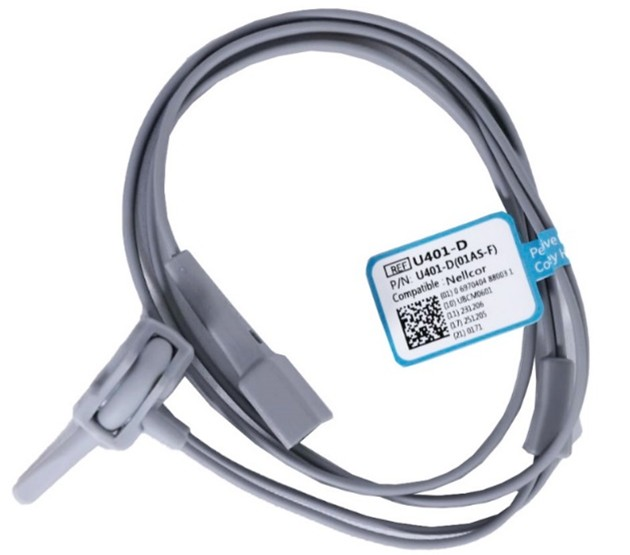
\includegraphics[width=0.5\linewidth]{img/sensor.jpg}
    \caption{Sensor U401-D utilizado para registrar los valores. Fuente: \href{https://www.humanhaim.com/product/sensor-de-oximetria-neo-sp02-7pin-u401-d01as-f/}{HumanHaim.}}
    \label{fig:sensor}
\end{figure}

\newpage

\textbf{PCB de la incubadora}

Contiene el circuito AFE4490 y un microcontrolador ESP32. El AFE es el encargado de amplificar, filtrar y digitalizar las señales analógicas provenientes del sensor óptico, mientras que el microcontrolador gestiona la comunicación con el exterior y la ejecución del firmware.

\begin{figure}[H]
    \centering
    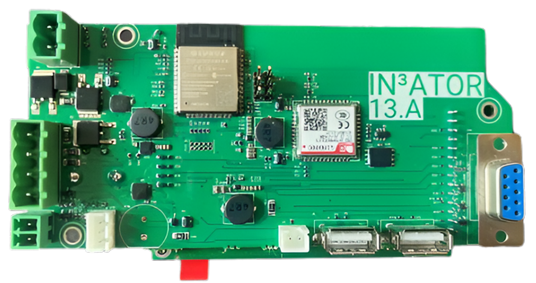
\includegraphics[width=0.75\linewidth]{img/PCB.png}
    \caption{Placa electrónica de la incubadora \textit{In$^3$ator}. \textit{Elaboración propia.}}
    \label{fig:PCB}
\end{figure}

    
\textbf{Programador EPS-Prog}

Permite cargar el firmware en el microcontrolador a través de un puerto de programación. Se conecta al ordenador mediante un adaptador micro-USB.

\begin{figure}[H]
    \centering
    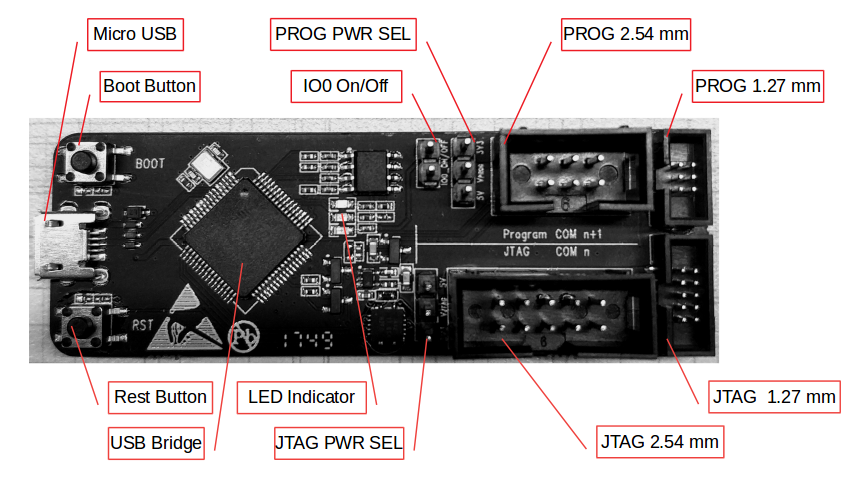
\includegraphics[width=0.7\linewidth]{img/EPS-prog.png}
    \caption{Programador a través del cual se transmiten los datos desde la placa al ordenador. Fuente: \href{https://docs.espressif.com/projects/esp-dev-kits/en/latest/other/esp-prog/user_guide.html}{Espressif.}}
    \label{fig:EPS-prog}
\end{figure}

\newpage

\textbf{Pulsioxímetros comerciales externos}

Utilizados como referencia para validar los resultados del sistema desarrollado:
    \begin{itemize}
        \item \textbf{AOJ-70C Berrcom (Amazon)}
        \begin{figure}[H]
            \centering
            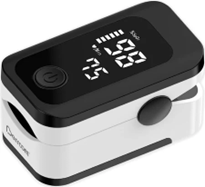
\includegraphics[width=0.3\linewidth]{img/pulsi1.png}
            \caption{Pulsioxímetro comercial 1 para validar los datos. Fuente: \href{https://www.amazon.es/}{Amazon.}}
            \label{fig:pulsi1}
        \end{figure}
        \item \textbf{VitalControl (LIDL)}
        \begin{figure}[H]
            \centering
            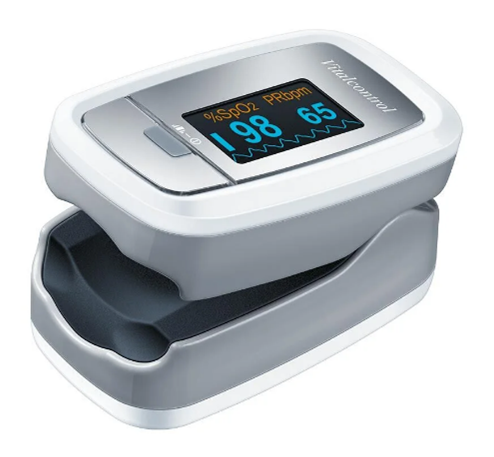
\includegraphics[width=0.35\linewidth]{img/pulsi2.png}
            \caption{Pulsioxímetro comercial 2 para validar los datos. Fuente: \href{https://www.amazon.es/}{Amazon.}}
            \label{fig:pulsi2}
        \end{figure}
    \end{itemize}


\subsubsection{Montaje del sistema}

\begin{enumerate}
    \item Se conecta la fuente de alimentación de 12V a un enchufe doméstico y se acopla un adaptador AC/DC, que convierte la corriente alterna en continua. Este se conecta a la entrada de alimentación de la PCB (ir al punto de conexión 1 de la imagen \ref{fig:PCBpartes}).
    \item El programador EPS-Prog se conecta al ordenador por USB y al microcontrolador en la PCB a través de los pines de programación(ir al punto de conexión 2 de la imagen \ref{fig:PCBpartes}). Una vez detectado por el portátil, permite cargar el firmware mediante PlatformIO.
    \item El sensor óptico U401-D se conecta a la PCB a través de un conector DB9 hembra (ir al punto de conexión 3 de la imagen \ref{fig:PCBpartes}). Durante las mediciones, se fija al dedo del usuario para asegurar un contacto adecuado con la piel.
    \begin{figure}[H]
        \centering
        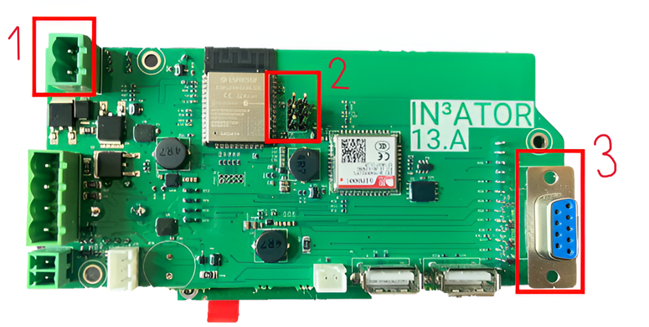
\includegraphics[width=0.85\linewidth]{img/PCBpartes.png}
        \caption{Partes de la PCB que se han utilizado para este proyecto concreto. \textit{Elaboración propia.}}
        \label{fig:PCBpartes}
    \end{figure}
    \item En la otra mano (o en otro dedo de la misma mano), se coloca un pulsioxímetro comercial. Sus lecturas se utilizan como referencia para registrar los valores de SpO$_2$ y frecuencia cardíaca en el nombre del archivo generado: \texttt{raw\_data\_SpO2\_HR.csv}.
\end{enumerate}

\begin{figure}[H]
    \centering
    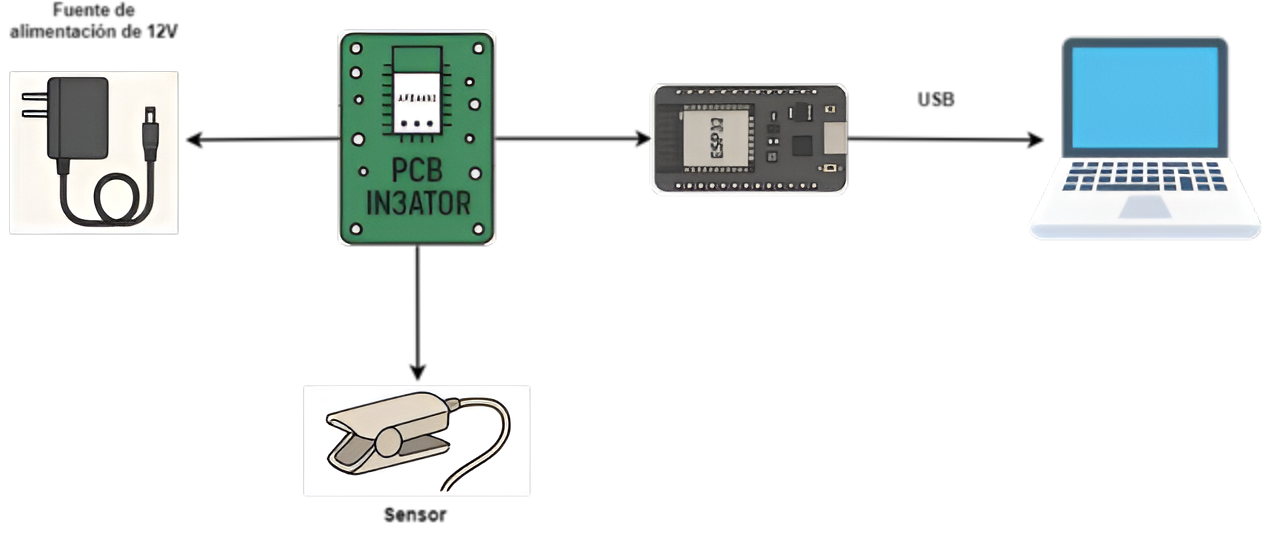
\includegraphics[width=0.95\linewidth]{img/flujo.png}
    \caption{Esquema de conexión para obtener los registros.\textit{Elaboración propia.}}
    \label{fig:flujo}
\end{figure}

\subsection{Software y lenguajes de programación}

Para la adquisición, análisis de los datos e implementación del código, se emplearon las siguientes herramientas de software:

\paragraph{Lenguajes utilizados}

\begin{itemize}
    \item \textbf{Python}: empleado para analizar los logs (registros), procesar las señales PPG y probar los algoritmos de estimación de los parámetros. 
    \item \textbf{C ++}: usado para desarrollar y modificar el firmware que corre en el microcontrolador.
    \item \textbf{LaTeX}: utilizado para la redacción de la memoria del TFG y los anexos técnicos, permitiendo una presentación adecuada.
\end{itemize}

\paragraph{Entornos de desarrollo}

\begin{itemize}
    \item \textbf{Jupyter Notebook}: entorno interactivo para el análisis exploratorio de datos, visualización y documentación del proceso.
    \item \textbf{Visual Studio Code}: entorno de desarrollo principal para trabajar con el firmware. 
\end{itemize}


\paragraph{Librerías de Python}\footnote{Cabe destacar que muchas de las librerías integradas en el entorno de desarrollo original (como PlatformIO en VS Code) ya estaban presentes en el firmware heredado del proyecto, por lo que no todas han sido incorporadas específicamente como parte de este trabajo. Se mencionan aquellas utilizadas en Python.}

\begin{itemize}
    \item \texttt{NumPy}, \texttt{Pandas}: para la manipulación de datos en formato CSV.
    \item \texttt{Matplotlib}, \texttt{Seaborn}: para la visualización de señales y tendencias.
    \item \texttt{SciPy}: para aplicar filtros digitales y detectar picos.
    \item \texttt{OpenCV} (en fase de pruebas): para el tratamiento de ruido y procesamiento de señales como si fueran imágenes.
\end{itemize}

\subsection{Otras herramientas empleadas}

\begin{itemize}
    \item \textbf{PlatformIO}: entorno de desarrollo para microcontroladores integrado en VS Code. Automatiza la gestión de bibliotecas, la compilación y la carga de firmware.
    \item \textbf{Drivers del EPS-Prog}: controladores VCP\footnote{Los controladores de puerto COM virtual (VCP) hacen que el dispositivo USB aparezca como un puerto COM adicional disponible para el PC.} necesarios para que el programador sea reconocido como puerto COM.
    \item \textbf{GitHub}: plataforma utilizada para el control de versiones, documentación y almacenamiento de código. Se gestionaron scripts, versiones del firmware, tareas, hitos y documentación asociada del proyecto.
    \item \textbf{Microsoft Word}: empleado durante las fases iniciales del proyecto para la toma de notas, redacción de borradores y estructuración de contenidos antes de pasarlo a LaTeX.
    \item \textbf{Draw.io (diagrams.net)}: utilizado para la creación de diagramas de bloques que representan los algoritmos, y esquemas funcionales que representan el flujo de la metodología y la arquitectura del sistema.

\end{itemize}


\section{Técnicas de procesamiento de señales}

Debido al enfoque del proyecto, se ha considerado necesario dedicar una sección específica a las técnicas de procesamiento de las señales empleadas.

El objetivo principal de este bloque es detallar los métodos aplicados para limpiar, transformar y analizar las señales PPG, así como los criterios seguidos para estimar los parámetros fisiológicos objetivo. A lo largo de esta sección se describen las distintas estrategias exploradas, su validación práctica sobre los datos reales adquiridos y la justificación técnica de las decisiones adoptadas para seleccionar los algoritmos finales.


Antes de proceder al diseño e implementación de los algoritmos de estimación, se realizó una fase de selección de las señales registradas. Con el objetivo de mejorar la precisión del análisis, se escogieron manualmente aquellas adquisiciones que presentaban señales estables, minimizando la presencia de artefactos de movimiento e interferencias lumínicas.\footnote{A pesar de realizar una selección previa, se seguían registrando señales que mostraban artefactos de distintos tipo, pero aun así se analizaron aquellas partes de la señal que podrían ofrecer información valiosa}

El análisis y desarrollo de estos algoritmos se llevó a cabo en Jupyter Notebook, y todos los scripts empleados se encuentran disponibles en el repositorio del proyecto para su consulta y replicación. Esta elección permitió trabajar en un entorno controlado, con el objetivo de experimentar con distintas estrategias de filtrado y estimación sin las limitaciones del microcontrolador.  

\subsection{Estimación de la frecuencia cardíaca}

La frecuencia cardíaca se estimó a partir de las señales PPG procedentes de los datos recogidos, explorando diferentes técnicas de procesamiento temporal y frecuencial. A lo largo de este apartado, se detallan los algoritmos evaluados, su implementación práctica y los criterios que guiaron la selección del método final.

El objetivo era seleccionar el algoritmo que ofreciera el mejor compromiso entre precisión, tolerancia frente al ruido y viabilidad de implementación en el microcontrolador del sistema.

Inicialmente, se visualizaron las señales gráficamente y se implementaron diferentes planteamientos fallidos \footnote{Aquellas pruebas con las que no se obtuvieron buenos resultados, serán nombradas en el \textit{anexo G} y están disponibles en el repositorio en el directorio de \texttt{pruebas} dentro del procesamiento de la frecuencia cardíaca.}.

En la fase posterior, se llevó a cabo una revisión de metodologías aplicadas en la literatura científica. Entre ellas destacan el algoritmo de detección de picos adaptativos \cite{9493400}, basado en el uso de un umbral adaptativo en función del ritmo cardíaco, y el método combinado de cruce de umbral y ventana deslizante descrito en la nota de aplicación de Renesas \cite{renesas2022ob1203}.
A partir de estas referencias, se implementaron y compararon diferentes enfoques en Jupyter Notebook, empleando como base los logs de adquisición propios. Los principales métodos evaluados fueron:


\begin{itemize}
    \item \textbf{AFE4403.ipynb}: basado en el artículo técnico de Texas Instruments sobre el AFE4403 \cite{oak2015how}. Se aplicaron filtros pasa-banda Butterworth y Savitzky-Golay para eliminar ruido y calcular la frecuencia cardíaca por separación entre picos.
    \begin{figure}[H]
        \centering
        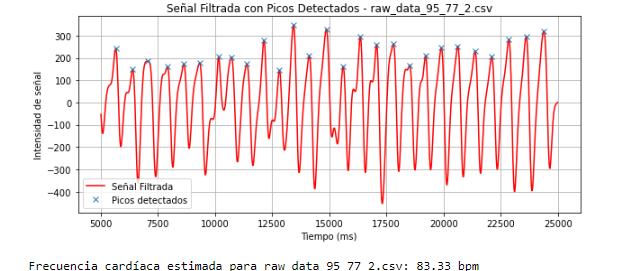
\includegraphics[width=0.85\linewidth]{img/AFE4403.png}
        \caption{Ejemplo de señal filtrada, aplicando el algoritmo del fichero \texttt{AFE4403.ipynb}. \textit{Elaboración propia.}}
        \label{fig:AFE4403}
    \end{figure}
    \item \textbf{AlgoritmoLigero.ipynb}: implementación del algoritmo de Vourvoulakis et al., del artículo \cite{9493400}, basado en umbrales adaptativos sobre las señales IR y RED.
    \begin{figure}[H]
        \centering
        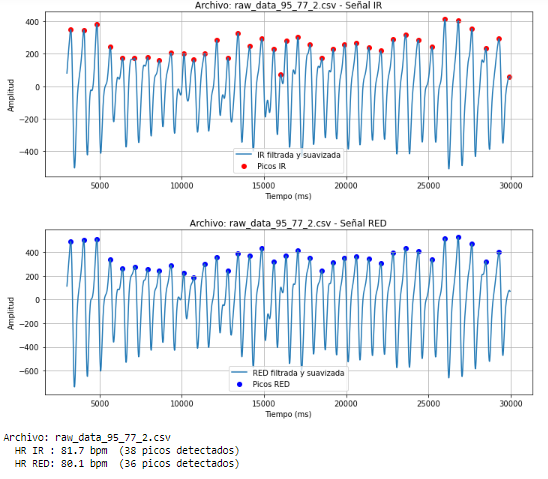
\includegraphics[width=0.85\linewidth]{img/Algoligero.png}
        \caption{Ejemplo de señal filtrada, aplicando el algoritmo del fichero \texttt{AlgoritmoLigero.ipynb}. \textit{Elaboración propia.}}
        \label{fig:AlgoLigero}
    \end{figure}
    \item \textbf{FFT.ipynb}: Este procedimiento no se basa en ningún artículo científico, si no que es un plantemiento que facilita la comprensión del tratamiento de la señal. Se trata de la estimación de la frecuencia cardíaca en el dominio de la frecuencia mediante Transformada Rápida de Fourier tras haber aplicado un filtro paso-bajo.
    \begin{figure}[H]
        \centering
        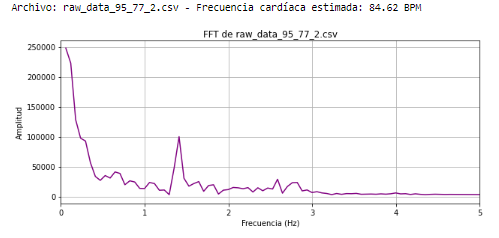
\includegraphics[width=0.85\linewidth]{img/FFT.png}
        \caption{Ejemplo de señal filtrada, aplicando el algoritmo del fichero \texttt{FFT.ipynb}. \textit{Elaboración propia}.}
        \label{fig:FFT}
    \end{figure}
    \item \textbf{procesamiento.ipynb}: procesamiento completo tras eliminación manual de segmentos inestables en los extremos de las señales, se utiliza un filtro Butterworth paso-bajo.
    \begin{figure}[H]
        \centering
        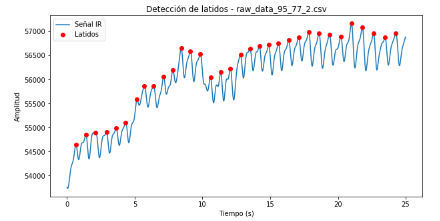
\includegraphics[width=0.85\linewidth]{img/procesamiento.png}
        \label{fig:FFT}
    \end{figure}
    \begin{figure}[H]
        \centering
        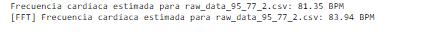
\includegraphics[width=0.85\linewidth]{img/procesamiento1.png}
        \caption{Ejemplo de señal filtrada, aplicando el algoritmo del fichero \texttt{procesamiento.ipynb}. \textit{Elaboración propia}.}
        \label{fig:FFT}
    \end{figure}
    \item \textbf{Pulsi\_comercial.ipynb}: simulación del funcionamiento de un pulsioxímetro comercial, con filtro paso-bajo Butterworth y estimación RR.
    \begin{figure}[H]
        \centering
        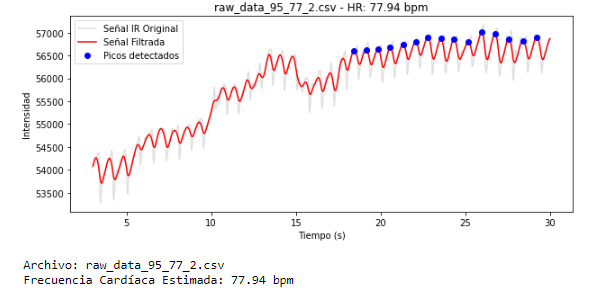
\includegraphics[width=0.85\linewidth]{img/pulsi_comercial.png}
        \caption{Ejemplo de señal filtrada, aplicando el algoritmo del fichero \texttt{pulsi\_comercial.ipynb}. \textit{Elaboración propia}.}
        \label{fig:pulsi_comercial}
    \end{figure}
    \item \textbf{spo2.ipynb}: detección de picos tras filtrado por media móvil y mediana.
    \begin{figure}[H]
        \centering
        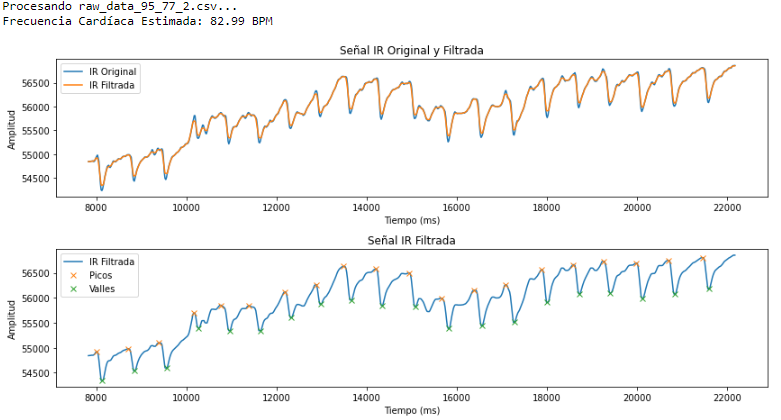
\includegraphics[width=0.75\linewidth]{img/spo2.png}
        \caption{Ejemplo de señal filtrada, aplicando el algoritmo del fichero \texttt{spo2.ipynb}. \textit{Elaboración propia}.}
        \label{fig:spo2}
    \end{figure}
    \item \textbf{temporal\_fft:} Se aplica un filtro pasabanda Butterworth de segundo orden, eliminando componentes de ruido fuera del rango fisiológico del pulso. Posteriormente, se utilizó la transformada rápida de Fourier para identificar la frecuencia dominante del espectro, que se tradujo a pulsaciones por minuto.
    \begin{figure}[H]
        \centering
        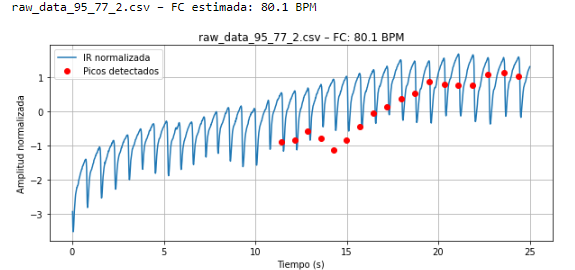
\includegraphics[width=0.85\linewidth]{img/temporal_fft.png}
        \caption{Ejemplo de señal filtrada, aplicando el algoritmo del fichero \texttt{temporal\_fft.ipynb}. \textit{Elaboración propia}.}
        \label{fig:temporal_fft}
    \end{figure}
\end{itemize}

Todas las imágenes mostradas corresponden a un mismo registro. Para ver los resultados de estos algoritmos sobre el resto de logs, consultar los notebooks correspondientes.

\subsubsection{Comparativa de métodos}

De entre todos los métodos analizados, se seleccionaron dos enfoques basados en el dominio temporal para su comparación detallada debido a la precisión de sus resultados:

\begin{enumerate}
    \item Algoritmo basado en media móvil + mediana + detección de picos (\texttt{spo2.ipynb}).
    \item Algoritmo basado en filtro Butterworth + detección de picos y eliminación de outliers (\texttt{pulsi\_comercial.ipynb}).
\end{enumerate}

\paragraph{Método 1: Filtro de media móvil y mediana.}

Este algoritmo se basa en un procesamiento sobre la señal IR corregida. El procedimiento comienza con una limpieza de los extremos del registro para eliminar los primeros y últimos segundos sobrantes (\(t_{\text{inicio}}\), \(t_{\text{fin}}\)) con el objetivo de descartar regiones inestables que puedan contener artefactos asociados al contacto inicial o la retirada del sensor.

\begin{itemize}
    \item La frecuencia de muestreo (\ref{eq:fs}) se estima a partir de la mediana del intervalo temporal (\ref{eq:mediana}) entre muestras consecutivas:
    \begin{equation}
        f_s = \frac{1}{\text{mediana}(\Delta t)} \quad
        \label{eq:fs}
    \end{equation}
    \begin{center}
        donde
    \end{center} \begin{equation}
        \quad \Delta t = \frac{t_{i+1} - t_i}{1000}
        \label{eq:mediana}
    \end{equation}
    \item Se aplica un filtro de media móvil de ventana \(M = 5\) (\ref{eq: media5}) para suavizar oscilaciones no fisiológicas de alta frecuencia:
    \begin{equation}
    IR_{\text{filtrada}}[n] = \frac{1}{5} \sum_{k=-2}^{2} IR[n+k]
    \label{eq: media5}
    \end{equation}
    \item A continuación, se aplica un filtro de mediana con una ventana también de 5 muestras, con el fin de eliminar picos de ruido que podrían confundirse con pulsos reales, conservando la morfología de los pulsos.
    \item La detección de pulsos se realiza a través de un algoritmo de búsqueda de máximos locales. En primer lugar, se identifican los picos como los puntos más altos de la señal filtrada, siempre que cumplan con una separación mínima entre sí. Posteriormente, se obtiene la posición de los valles aplicando el mismo algoritmo sobre la señal invertida (\(-IR_{\text{filtrada}}\)), permitiendo localizar los mínimos locales con el mismo criterio. Para evitar contar múltiples picos dentro de un mismo latido, se impone una distancia mínima de 0.5 segundos (\ref{eq:dist}) entre detecciones consecutivas:

    \begin{equation}
    \text{distancia mínima} = 0.5 \cdot f_s
    \label{eq:dist}
    \end{equation}
    \item Finalmente, se calcula la frecuencia cardíaca (\ref{eq: HR2}) a partir de la media de los intervalos de tiempo entre valles consecutivos:
    \begin{equation}
    HR = \frac{60}{\text{media}(\Delta t_{\text{valles}})}
    \label{eq: HR2}
    \end{equation}
\end{itemize}

\begin{figure}[H]
    \centering
    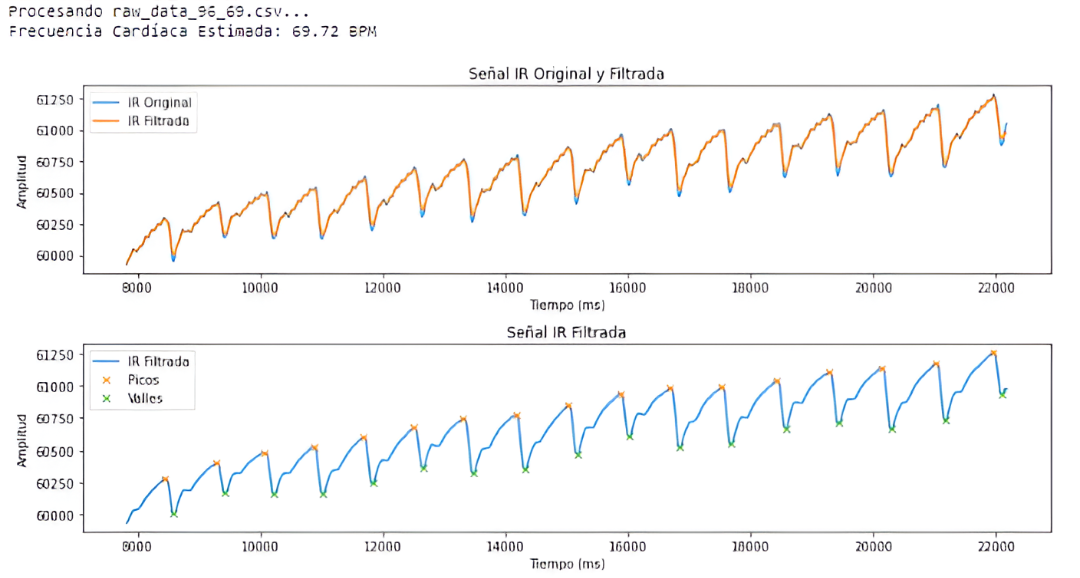
\includegraphics[width=0.95\linewidth]{img/spo2_2.png}
    \caption{Ejemplo de aplicar el algoritmo mencionado sobre otro log diferente. \textit{Elaboración propia.}}
    \label{fig:spo2_2}
\end{figure}

Este método se ha escogido por su eficacia y destaca por su simplicidad y eficiencia computacional, por lo que resulta adecuado para implementarlo más adelante en el firmware original.


\paragraph{Método 2: Filtro Butterworth pasa-bajo y detección de picos con eliminación de outliers.}

Este segundo método se basa en aplicar un filtrado digital suave, seguido de una detección de picos sobre la señal IR.

\begin{itemize}
    \item Se parte de los datos previamente limpiados (archivos CSV en la carpeta \texttt{Datos\_limpios}), con la señal IR.
    \item La señal IR se suaviza utilizando un filtro digital pasa-bajo Butterworth de orden 3 y frecuencia de corte \( f_c = 3{,}5\,\text{Hz} \). El filtrado se aplica en ambos sentidos mediante \texttt{filtfilt}. Este método localiza los máximos locales que cumplen dos condiciones fisiológicas:
\begin{itemize}
    \item Se exige una altura mínima adaptativa (\ref{eq: height}), definida como el percentil 80 de la señal. Esto permite ignorar oscilaciones menores y centrarse solo en los pulsos más elevados:
    \begin{equation}
    \texttt{height} = \text{percentil}_{80}(\text{señal filtrada})
    \label{eq: height}
    \end{equation}
    \item Se impone una separación mínima entre pulsos de 18 muestras, equivalente a 0,18 segundos con un muestreo de 100 Hz. Esto limita la detección a un máximo fisiológico de aproximadamente 333 latidos por minuto:
    \begin{equation}
    \texttt{distance} = 18 \text{ muestras } \Rightarrow HR_{\text{máx}} \approx \frac{60}{0{,}18} \approx 333\,\text{bpm}
    \end{equation}
\end{itemize}
    \item A partir de los picos detectados, se calculan los intervalos RR:
    \begin{equation}
    \Delta t_i = t_{i+1} - t_i
    \end{equation}
    \item Para evitar que errores puntuales afecten al resultado, se eliminan los intervalos entre pulsos RR que se alejan demasiado del comportamiento normal. Para ello, se aplica el criterio del rango intercuartílico (IQR), que descarta los valores demasiado pequeños o demasiado grandes respecto a la mayoría. En lugar de usar el valor típico de 1.5, se ha optado por un umbral más estricto de 1.2, lo que ayuda a reducir falsos positivos en la estimación de la frecuencia cardíaca:
    \begin{equation}
    \Delta t \in [Q_1 - 1{,}2 \cdot IQR,\ Q_3 + 1{,}2 \cdot IQR]
    \end{equation}
    \item Finalmente, se estima la frecuencia cardíaca (\ref{eq:HR3}) a partir del intervalo medio entre picos válidos:
    \begin{equation}
    HR = \frac{60}{\text{media}(\Delta t_{\text{filtrados}})}
    \label{eq:HR3}
    \end{equation}
\end{itemize}

\begin{figure}[H]
    \centering
    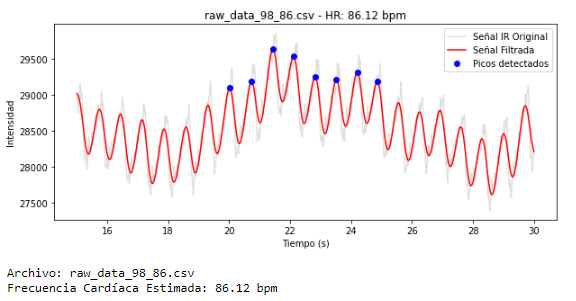
\includegraphics[width=0.85\linewidth]{img/pulsicomercial.png}
    \caption{Aplicación del algoritmo sobre señal real IR. En rojo la señal filtrada, en azul los picos detectados. \textit{Elaboración propia.}}
    \label{fig:pulsicomercial}
\end{figure}

Gracias al filtrado y a la detección adaptativa de picos, este método permite obtener estimaciones bastante fiables de la frecuencia cardíaca. Aun así, algunas de las funciones que utiliza, como \texttt{filtfilt} (para filtrar en ambos sentidos) o el cálculo de percentiles, son difíciles de trasladar tal cual al firmware, ya que habría que programarlas desde cero en C++. 


\paragraph{Selección final:}

Para seleccionar el mejor enfoque, se estudió el tiempo de ejecución de ambos filtros (sobre los logs de 60Hz de frecuencia)\footnote{Se puede revisar esta comprobación dentro del repositorio en el fichero \texttt{benchmark\_filtros.ipynb}, del directorio de procedimiento} y aunque resultó que el de menor tiempo computacional fue el filtro Butterworth, se optó finalmente por el algoritmo basado en filtro de media móvil. Si bien el método Butterworth ofrecía mejor rendimiento ante señales contaminadas, el hecho de utilizar funciones específicas de Python, lo hacía menos adecuado para su implementación en el microcontrolador actual.



\subsection{Estimación de SpO$_2$}

Al igual que en el caso de la frecuencia cardíaca, la estimación de la saturación de oxígeno en sangre requirió una fase exploratoria inicial. En ella se llevaron a cabo pruebas sobre los datos adquiridos, experimentando con técnicas de filtrado, métodos alternativos y ajustes de preprocesamiento. Estas pruebas se documentan en los notebooks correspondientes, disponibles en el repositorio del proyecto.

Los métodos principales considerados para la estimación de SpO$_2$ son los siguientes:

\paragraph{Método 1: \texttt{spo\_algo\_v4.ipynb}, Estimación mediante algoritmo adaptado del firmware.}

Este método representa una de las versiones desarrolladas a partir de la función \texttt{spo2\_algorithm.cpp} incluida en el archivo \texttt{SPO2.cpp} del firmware \textbf{original} de la incubadora. Dicho algoritmo estaba poco optimizado y no era fácilmente validable desde un entorno externo, ya que estaba integrado con el resto del sistema embebido. Por ello, se adaptó su lógica al entorno Python, lo que permitió visualizar sus resultados y validar su comportamiento sobre los datos adquiridos en las pruebas reales.

Aunque el firmware original implementa el cálculo de SpO$_2$ mediante una tabla de búsqueda (LUT, Look-Up-Table), en el propio archivo se encuentra comentada una fórmula alternativa cuadrática (\ref{eq:cuadratica}) que permite estimar la saturación directamente a partir del ratio de absorciones. Esta fórmula es la que se ha empleado en este método por su simplicidad, continuidad y buena aproximación dentro del rango fisiológico normal.

La fórmula:

\begin{equation}
SpO_2 = -45.060 \cdot R^2 + 30.354 \cdot R + 94.845
\label{eq:cuadratica}
\end{equation}

Esta expresión se obtiene a partir de regresiones cuadráticas realizadas sobre datos experimentales. Es decir, se mide el ratio \( R \) de absorción para diferentes personas o simulaciones, y se ajusta una curva que relacione ese ratio con el valor de SpO$_2$ medido por un pulsioxímetro de referencia. El resultado es una fórmula que permite estimar directamente la saturación a partir del ratio sin necesidad de tablas discretas.

El procedimiento aplicado fue el siguiente:

\begin{itemize}
    \item Se parte de los datos crudos adquiridos por el sensor, correspondientes a las intensidades de luz detectadas por los canales IR y RED.
    \item Se calcula la media de cada señal (\ref{eq:media}) para estimar su componente continua o de fondo (DC). Esto equivale a encontrar el nivel base de la señal:
    \begin{equation}
    \text{mean}_{IR} = \overline{IR}, \quad \text{mean}_{RED} = \overline{RED}
    \label{eq:media}
    \end{equation}
    \item A continuación, se resta esa media a cada señal para obtener su componente alterna (\ref{eq:AC}), que representa la parte pulsátil:
    \begin{equation}
    AC_{IR} = IR - \text{mean}_{IR}, \quad AC_{RED} = RED - \text{mean}_{RED}
    \label{eq:AC}
    \end{equation}
    \item Para cuantificar la amplitud de esa señal alterna, se calcula la \textbf{raíz cuadrada media (RMS)} de cada canal:
    \begin{equation}
    RMS_{IR} = \sqrt{\frac{1}{n} \sum_{i=1}^{n} (AC_{IR}[i])^2}, \quad RMS_{RED} = \sqrt{\frac{1}{n} \sum_{i=1}^{n} (AC_{RED}[i])^2}
    \label{eq:RMS}
    \end{equation}
    \item Con esos valores se calcula un ratio que compara la absorción de las dos longitudes de onda:
    \begin{equation}
    R = \frac{RMS_{RED} / \text{mean}_{RED}}{RMS_{IR} / \text{mean}_{IR}}
    \end{equation}
    \item Finalmente, se aplica la fórmula cuadrática ya mencionada para obtener la estimación del valor global de SpO$_2$ en el registro analizado.
\end{itemize}

\begin{figure}[H]
    \centering
    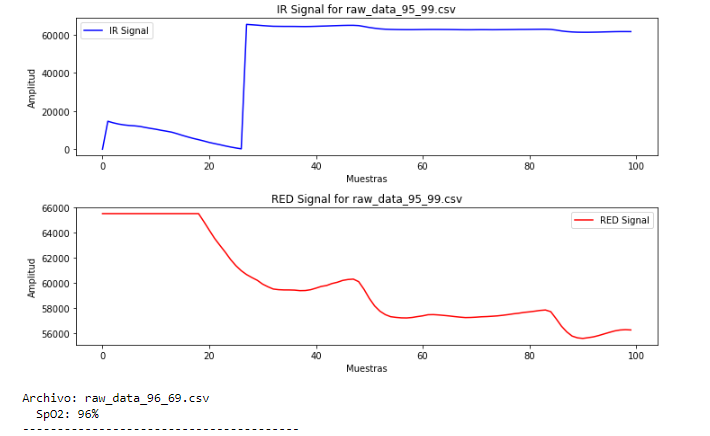
\includegraphics[width=0.85\linewidth]{img/spo2algo.png}
    \caption{Aplicación del algoritmo a los datos crudos según el archivo \texttt{spo\_algo\_v4.ipynb}. \textit{Elaboración propia.}}
    \label{fig:spo2algo}
\end{figure}

Aunque este método resulta sencillo de implementar y computacionalmente eficiente, los resultados obtenidos durante su validación sobre las señales reales del sistema no fueron completamente satisfactorios. En concreto, en algunos registros se observaron desviaciones notables respecto a los valores de referencia, con estimaciones de SpO$_2$ que resultaban poco realistas.

Estas limitaciones pueden deberse a varios factores: la sensibilidad del ratio \( R \) a pequeñas variaciones en la señal, y el uso de una fórmula empírica que no está ajustada específicamente a las condiciones del sensor empleado. Aun así, este método sirvió como base para compararlo con enfoques desarrollados posteriormente.


\paragraph{Método 2: \texttt{tabla\_LUT.ipynb}, Estimación basada en generación de tabla LUT.}

Este segundo método parte de una idea diferente al algoritmo del firmware. En lugar de aplicar directamente una fórmula empírica fija como en el método anterior, aquí se propone construir una tabla LUT personalizada, generada a partir de los datos reales adquiridos durante las pruebas del sistema. El objetivo es observar la relación entre el ratio óptico \(R\) calculado a partir de las señales y el valor de SpO$_2$ que se había registrado con un pulsioxímetro comercial como referencia.

El procedimiento seguido en este notebook fue el siguiente:

\begin{itemize}
    \item Se recorrieron todos los archivos CSV con datos limpios.
    \item Para cada archivo, se cargaron las señales IR y RED, y se calcularon sus componentes AC (desviación típica) y DC (media). Con esos valores se estimó el ratio óptico mediante:
    \begin{equation}
    R = \frac{AC_{RED} / DC_{RED}}{AC_{IR} / DC_{IR}}
    \end{equation}
    \item Se almacenó, para cada archivo, el valor de \(R\) y su correspondiente SpO$_2$ de referencia.
    \begin{figure}[H]
        \centering
        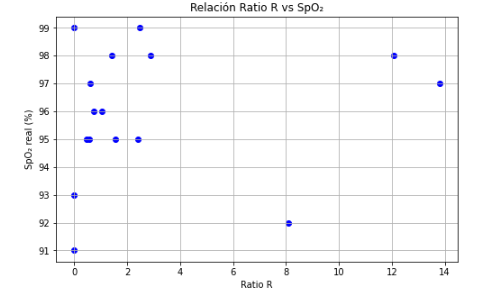
\includegraphics[width=0.75\linewidth]{img/LUT2.png}
        \caption{Gráfico de dispersión que relaciona los valores de R con los de SpO$_2$ a partir del archivo \texttt{tabla\_LUT.ipynb}. \textit{Elaboración propia.}}
        \label{fig:LUT2}
    \end{figure}
    \item Finalmente, se representaron gráficamente estos valores (figura \ref{fig:LUT2}) y se detectaron algunos puntos con ratios extremos (muy altos o iguales a cero). Tras este filtrado, se obtuvo una tabla LUT con pares de valores \((R, \text{SpO}_2)\) válidos, que permite visualizar la tendencia real entre el ratio óptico y la saturación.
    \begin{figure}[H]
        \centering
        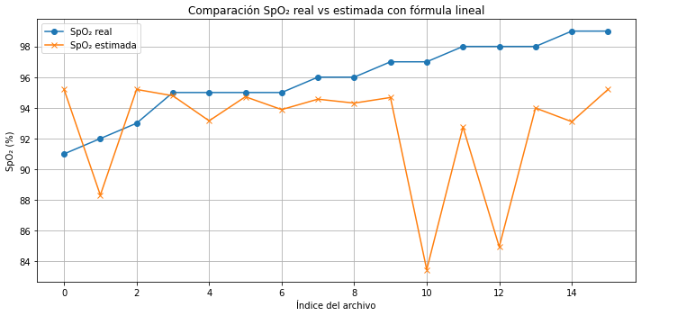
\includegraphics[width=0.85\linewidth]{img/LUT1.png}
        \caption{Comparación de los resultados con los valores de SpO$_2$ de referencia. \textit{Elaboración propia.}}
        \label{fig:LUT1}
    \end{figure}
\end{itemize}

Esta tabla se puede utilizar como base para futuros modelos personalizados (por ejemplo, una regresión lineal o una interpolación), o incluso para crear una LUT discreta implementable en firmware. El enfoque permite adaptar la estimación de SpO$_2$ al comportamiento real del sensor en el sistema desarrollado y tiene la ventaja de apoyarse directamente en datos experimentales propios.

No obstante, durante su ejecución se detectaron varios registros con valores erróneos o inconsistentes (por ejemplo, ratios iguales a cero o superiores a 8), que indican la sensibilidad de este método a errores de adquisición o ruido. También es importante destacar que para que esta opción sea fiable, es necesario tener un mayor número de logs o registros.


\paragraph{Método 3: \texttt{Paper\_CS.ipynb}: Estimación mediante regresión lineal ajustada.}

Este método propone una estrategia basada en aprendizaje automático sencillo: en lugar de utilizar una fórmula empírica genérica o una tabla LUT fija, se ajusta un modelo de regresión lineal personalizado utilizando exclusivamente los datos reales obtenidos durante las pruebas del sistema. Se ha tomado de base un artículo \cite{mohan2010blood}.

La idea es la siguiente: para cada archivo de registro de señales PPG (IR y RED), se calcula el ratio óptico \( R \) a partir del cociente entre las componentes pulsátiles (AC) de ambas señales, corregidas por sus respectivas componentes continuas (DC). La señal se corrige previamente restando la luz ambiental (\texttt{AMB\_IR} y \texttt{AMB\_RED}), y se calcula la RMS (\ref{eq:RMS2}) de las señales corregidas:

\begin{equation}
R = \frac{RMS_{RED}}{RMS_{IR}} \quad \text{donde   }   RMS = \sqrt{\frac{1}{n} \sum_{i=1}^{n} (x[i])^2}
\label{eq:RMS2}
\end{equation}

Luego, se toma como variable dependiente el valor real de SpO$_2$ anotado en el nombre del archivo (medido con un pulsioxímetro comercial) y se entrena un modelo de regresión lineal con la forma:

\begin{equation}
SpO_2 = m \cdot R + b
\end{equation}

Tras el ajuste, se obtuvo el siguiente modelo:

\begin{equation}
SpO_2 = -0.9560 \cdot R + 96.66
\end{equation}

\begin{figure}[H]
    \centering
    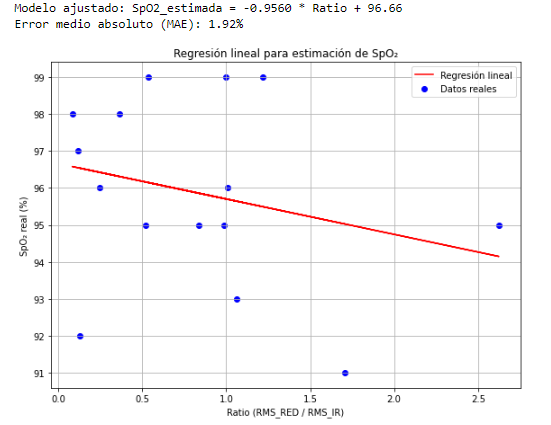
\includegraphics[width=0.75\linewidth]{img/modelo.png}
    \caption{Modelo de regresión obtenido con los datos propios para conseguir los valores \textit{a} y \textit{b} según el archivo \texttt{Paper\_CS.ipynb}. \textit{Elaboración propia.}}
    \label{fig:modelo}
\end{figure}

Este modelo fue validado con los datos disponibles, obteniendo un error medio absoluto (MAE) de 1.92 puntos porcentuales (figura \ref{fig:modelo}), lo que indica una buena capacidad de estimación promedio en las condiciones de adquisición empleadas.


Este método tiene la ventaja de estar ajustado directamente a las características reales del sistema, y permite una implementación sencilla en firmware (como una ecuación lineal). Además, ofrece una interpretación clara: a mayor ratio \( R \), menor saturación estimada, lo cual coincide con el comportamiento fisiológico esperado.

No obstante, es importante señalar que la calidad del ajuste depende fuertemente de la calidad y representatividad de los datos usados. En este caso, el modelo ha sido ajustado únicamente con señales limpias y valores de referencia de un único usuario, por lo que su generalización a otros pacientes o condiciones clínicas no ha sido evaluada.

\paragraph{Método 4: \texttt{uch\_spo2\_table.ipynb}: Generación personalizada de tabla LUT tipo firmware.}

Este método tiene como objetivo replicar el funcionamiento del algoritmo del firmware original, que utiliza una tabla de búsqueda (\texttt{uch\_spo2\_table}) para estimar el valor de SpO$_2$ a partir del ratio óptico \( R \). Sin embargo, en lugar de utilizar la tabla precalibrada incluida en el código fuente, en este caso se genera una LUT personalizada basada en los datos reales adquiridos durante el desarrollo del proyecto.

Este método se diferencia del anterior (basado en una LUT visual) en que, en lugar de almacenar valores de SpO$_2$ para cada índice, busca una expresión matemática directa que relacione el ratio óptico con la saturación.


El proceso seguido fue el siguiente:

\begin{itemize}
    \item Se recorrieron los archivos CSV con datos limpios, en los que el valor de SpO$_2$ real se extraía del nombre del archivo.
    \item Para cada archivo, se calcularon las señales corregidas (\texttt{IR} - \texttt{AMB\_IR} y \texttt{RED} - \texttt{AMB\_RED}), y se obtuvieron sus componentes AC y DC.
    \item Se calculó el ratio óptico como:
    \begin{equation}
    R = \frac{AC_{RED}/DC_{RED}}{AC_{IR}/DC_{IR}}, \quad \text{donde }
    \end{equation}
    \begin{equation}
    AC = \max(\text{señal}) - \min(\text{señal},) \quad DC = \overline{\text{señal}}
    \end{equation}
    \item El valor del ratio se multiplicó por 100 y se redondeó para usarlo como índice de acceso a la tabla LUT.
    \item Para cada índice (de 0 a 183), se almacenaron los valores de SpO$_2$ reales correspondientes, y se calculó su media.
    \item Los índices sin datos suficientes fueron rellenados mediante interpolación lineal, asegurando una tabla continua sin saltos muy grandes. El resultado fue una tabla de 184 posiciones que asigna un valor de SpO$_2$ a cada rango de ratio observado.

\end{itemize}

Esta tabla fue visualizada y validada gráficamente (figura \ref{fig:uch_spo2}), mostrando el comportamiento fisiológico esperado. El método permite estimar directamente el valor de SpO$_2$ de cualquier nuevo registro utilizando una única operación de acceso a tabla (más interpolación si se desea). No obstante, también hereda las limitaciones mencionadas en otros métodos.

\begin{figure}[H]
    \centering
    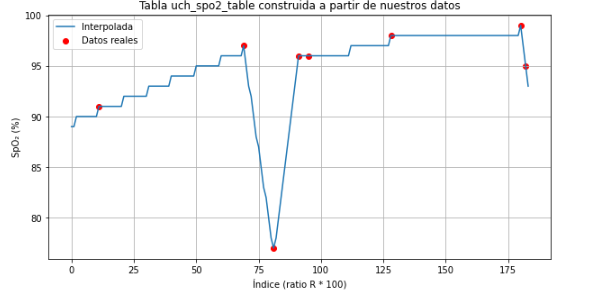
\includegraphics[width=0.85\linewidth]{img/uch_spo2.png}
    \caption{Gráfico de la tabla construida a partir de los datos propios a partir del archivo \texttt{uch\_spo2\_table.ipynb}. \textit{Elaboración propia}.}
    \label{fig:uch_spo2}
\end{figure}


\paragraph{Selección final:}

De entre los métodos evaluados, el que mostró mejor equilibrio entre precisión, estabilidad y viabilidad de implementación en firmware fue el \textbf{Método 4}, basado en una tabla de búsqueda discreta generada a partir de los datos reales adquiridos con el sistema. Este método permitió capturar la relación entre el ratio óptico \(R\) y la saturación de oxígeno SpO$_2$ directamente desde los experimentos realizados, evitando el uso de fórmulas genéricas o calibraciones externas.

Aunque otros enfoques como la fórmula cuadrática (Método 1) o la regresión lineal ajustada (Método 3) ofrecían ventajas en términos de continuidad o simplicidad matemática, el uso de una LUT precalculada resultó menos sensible frente a señales con ruido. Además, la implementación tipo firmware de esta tabla permite estimaciones rápidas y estables sin necesidad de cálculos complejos en tiempo real.

Por tanto, la versión final del firmware emplea este método LUT, lo que asegura una estimación de SpO$_2$ coherente con el comportamiento real del sensor y viable dentro de las limitaciones del sistema.

\vspace{0.4cm}
\noindent
\textbf{Resumen comparativo y criterios de selección}

Más allá de la precisión teórica, la elección del algoritmo final tuvo en cuenta factores como la estabilidad ante ruido y la viabilidad de implementación en sistemas embebidos. En la Tabla~\ref{tab:resumen_spo2} se sintetizan las principales características de cada enfoque probado.

\begin{table}[H]
\centering
\footnotesize
\renewcommand{\arraystretch}{1.2}
\begin{tabular}{|p{2.6cm}|p{4.4cm}|p{4.4cm}|}
\hline
\textbf{Método} & \textbf{Ventajas} & \textbf{Limitaciones} \\
\hline
\textbf{1. Fórmula cuadrática} & Continuo, simple de aplicar & Sensible al ruido, desviaciones fisiológicas \\
\hline
\textbf{2. LUT visual} & Ajustado a datos reales, interpretable & No implementable directamente, requiere muchos datos \\
\hline
\textbf{3. Regresión lineal} & Ecuación directa y calibrable & Dependiente del conjunto de entrenamiento, poco robusto \\
\hline
\rowcolor{gray!20}
\textbf{4. LUT tipo firmware} & Robusto, eficiente, fácil de integrar & Precisión limitada al conjunto de calibración inicial \\
\hline
\end{tabular}
\caption{Resumen de los métodos de estimación de SpO$_2$ evaluados. \textit{Elaboración propia.}}
\label{tab:resumen_spo2}
\end{table}


\subsection{Implementación en el firmware}

Una vez identificados los algoritmos más adecuados para la estimación de la frecuencia cardíaca y la saturación de oxígeno en entorno Python, se procedió a su adaptación al firmware del sistema embebido. Esta etapa supuso un reto técnico importante, ya que implicaba trasladar algoritmos previamente validados en un entorno conocido a un código escrito en un lenguaje poco trabajado durante el grado, y además hacerlo respetando la estructura existente del firmware, con múltiples archivos interdependientes y funciones ya implementadas.

El objetivo era lograr que el microcontrolador fuera capaz de procesar los datos en tiempo real y emitir directamente por puerto serie los valores de frecuencia cardíaca y SpO$_2$, eliminando la necesidad de postprocesamiento en PC. Para ello, fue necesario reestructurar parte del código original, optimizar las funciones de cálculo y rediseñar el flujo de adquisición y salida de datos.

La Figura~\ref{fig:flujo_firmware} muestra el esquema general del nuevo flujo de procesamiento de señal implementado dentro del firmware.


\begin{figure}[H]
    \centering
    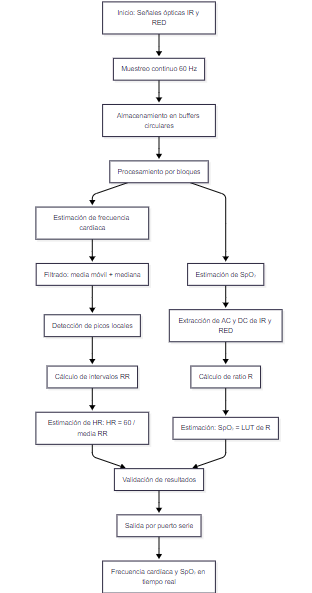
\includegraphics[width=0.6\linewidth]{img/flujo_firmware.png}
    \caption{Diagrama de flujo que representa el código implementado en el firmware. \textit{Elaboración propia.}}
    \label{fig:flujo_firmware}
\end{figure}

\newpage

\paragraph{Estimación de la frecuencia cardíaca.}

La estimación de la frecuencia cardíaca se implementa dentro de la función \texttt{estimate\_spo2()} del archivo \texttt{SPO2.cpp}, que procesa bloques de datos adquiridos por el sensor. El firmware trabaja sobre la señal IR, almacenada en un buffer circular \footnote{Un \textit{buffer circular} es una estructura de datos que almacena una cantidad fija de elementos y, cuando se llena, comienza a sobrescribir los datos más antiguos con los nuevos. Permite procesar continuamente señales, por eso, se suele utilizar en sistemas en tiempo real.}
de 128 posiciones, actualizado en tiempo real a una frecuencia de muestreo de 100 Hz. Esto permite mantener siempre una ventana de datos recientes sin necesidad de desplazar manualmente los elementos del buffer.

La señal IR se centra restando su media y se invierte, de modo que los valles fisiológicos (mínimos de absorción) se transforman en picos. Posteriormente, se suaviza con una media móvil de cuatro muestras, y sobre esa señal invertida se aplica un umbral adaptativo para detectar los picos correspondientes a los valles reales.

\begin{figure}[H]
    \centering
    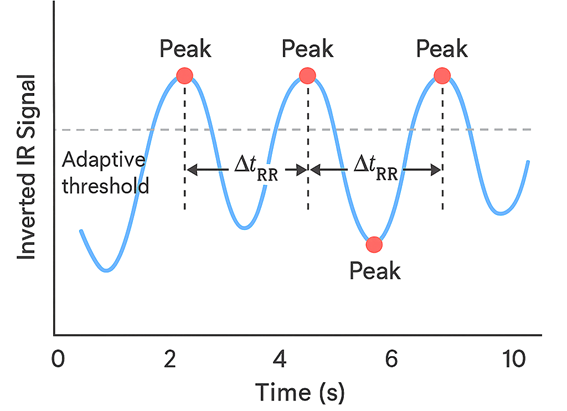
\includegraphics[width=0.5\linewidth]{img/fc_algo.png}
    \caption{Detección de picos locales en una señal pulsátil y cálculo de intervalos RR. \textit{Elaboración propia.}}
    \label{fig:enter-label}
\end{figure}

Si se detectan al menos dos valles válidos, se calcula la frecuencia cardíaca estimando el intervalo medio entre ellos ($\Delta t_{\text{RR}}$), y aplicando la fórmula:

\begin{equation}
\text{HR} = \frac{60}{\text{media}(\Delta t_{\text{RR}})}
\end{equation}

donde:

\begin{equation}
\Delta t_i = \frac{t_{i+1} - t_i}{f_m}
\end{equation}

y $f_m$ es la frecuencia de muestreo en Hz. El resultado final se valida para asegurar que se encuentra dentro del rango fisiológico razonable (entre 40 y 220 BPM). Si no cumple con esta condición, se descarta.


\paragraph{Estimación de la saturación de oxígeno.}

La estimación de SpO$_2$ se realiza en la misma función \texttt{estimate\_spo2()}, reutilizando los valles previamente detectados en la señal IR para dividir la señal en ciclos pulsátiles (es decir, segmentos entre dos latidos consecutivos). En cada ciclo se calcula la componente AC y la componente DC tanto de la señal RED como de la IR, aplicando las siguientes fórmulas:

\begin{equation}
AC = \max(x) - \min(x)\end{equation}\begin{equation} \qquad DC = \max(x)
\end{equation}

Con estos valores se calcula el \textit{ratio óptico} $R$, utilizando la siguiente expresión:

\begin{equation}
R = \frac{AC_{\text{RED}} \cdot DC_{\text{IR}} \cdot 100}{AC_{\text{IR}} \cdot DC_{\text{RED}}}
\end{equation}

Este cálculo se repite para un máximo de cinco ciclos válidos. Un ciclo se considera válido si las componentes AC y DC superan unos umbrales mínimos predefinidos, que garantizan que la señal no esté afectada por ruido o por un mal contacto del sensor.

Una vez obtenidos hasta cinco valores válidos de \(R\), estos se ordenan y se toma la mediana, ya que es menos sensible a valores atípicos provocados por artefactos de movimiento o interferencias.

El sistema emplea una tabla LUT con 184 posiciones. El valor de \(R\) se redondea al entero más próximo y se utiliza como índice para consultar el valor correspondiente de SpO\textsubscript{2} en dicha tabla:


\begin{equation}
\text{SpO}_2 = \text{LUT}[R]
\end{equation}

El valor estimado se valida asegurando que se encuentra dentro del rango fisiológico razonable (85\,\%–100\,\%); en caso contrario, se descarta.



